\documentclass[12pt,a4paper]{article}
\usepackage[latin1]{inputenc}
\usepackage[T1]{fontenc} 
\usepackage[francais, english]{babel} 
\usepackage{amsmath, amsthm}
\newtheorem{theorem}{Theorem}
\newtheorem{proposition}{Proposition}
\newtheorem{lemma}{Lemma}
\newtheorem*{proof*}{Proof}
\newtheorem{definition}{Definition}

\newtheorem{exercise}{Exercise}
\newtheorem{question}{Question}

\newtheorem{example}{Example}

\newtheorem{remark}{Remark}

\usepackage[a4paper,left=2cm, right=2cm,top=3cm,bottom=3cm]{geometry}
\usepackage{cancel}
\usepackage{bm}
\usepackage{amssymb,amsfonts}
\usepackage{mathrsfs}
\usepackage{color}
%\usepackage{hyperref}
\usepackage{dsfont}
\usepackage{graphicx}
\usepackage{algorithmicx}
\usepackage[ruled]{algorithm}
\usepackage{algpseudocode}
\usepackage{marginnote}
\newcommand{\Ptr}{\mathcal P^{\rm tr}}
\newcommand{\tr}{{\rm tr}}
\newcommand{\N}{\mathbb N}
\newcommand{\calN}{\mathcal N}
\newcommand{\bP}{\bold P}
\newcommand{\calK}{\mathcal K}
\newcommand{\calF}{\mathcal F}
\newcommand{\calH}{\mathcal H}
\newcommand{\calP}{\mathcal P}
\newcommand{\calC}{\mathcal C}
\newcommand\red[1]{\textcolor{red} {#1} }
\newcommand{\R}{\mathbb R}
\newcommand{\bX}{\bar X}
\newcommand{\Ktr}{\calK^{\rm tr}}
\title{ \bfseries \Huge {Handout 2: Markov chains}} 
\date{Due date : }       
\vspace{-1cm}        
\newcounter{num}  % Create a new counter for paragraphs

\setcounter{num}{1}  % Start the paragraph counter at 1
\begin{document}
	\maketitle
	\paragraph{Exercise \thenum.}%(Stationary distribution)
		Consider the Markov chain shown below, where $0 < p < 1$.
		\begin{figure}[h!]
			\begin{center}
				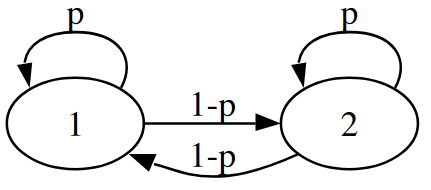
\includegraphics[width = .25\textwidth]{images/markov_p_1-p.png}
			\end{center}
		\end{figure}
		\begin{enumerate}
			\item Write down the transition matrix Q for this chain.
			\item Find the stationary distribution of the chain.
			\item What is the limit of $Q_n$ as $n\rightarrow\infty$?
		\end{enumerate} 
		
	
	\stepcounter{num} 
\paragraph{Exercise \thenum.} %(Stationary distribution)
	Consider the Markov chain shown below, with state space $\{1, 2, 3, 4\}$.
	\begin{figure}[h!]
		\begin{center}
			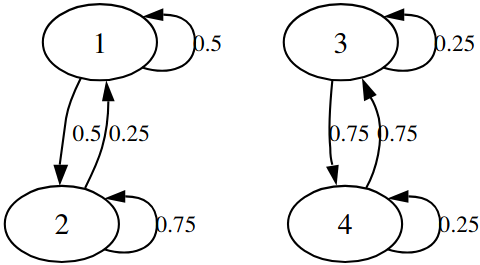
\includegraphics[width = .35\textwidth]{images/markov_2.png}
		\end{center}
	\end{figure}
	\begin{enumerate}
	\item Write down the transition matrix Q for this chain.
	\item Which states (if any) are recurrent? Which states (if any) are transient?
	\item Find two different stationary distributions for the chain.
	\end{enumerate} 


	\stepcounter{num} 
\paragraph{Exercise \thenum.}% (Stationary distribution)
	Consider a Markov chain with transition matrix
	$$P = \left(
	\begin{matrix}
		0.4 &0.6& 0& 0\\
		0.6& 0.4& 0 &0\\
		0& 0 &0.5 &0.5\\
		0 &0 &0.2 &0.8\\
	\end{matrix}
	\right)
	$$
	\begin{enumerate}
		\item States $i$ and $j$ communicate if $i$ is accessible from $j$ and $j$ is accessible from $i$. 
		Find all its communication classes.
		\item Given
		$$
		\underset{n\rightarrow \infty}{\rm lim} P^n = 
		 \left(
		\begin{matrix}
			0.5 &0.5& 0& 0\\
			0.5& 0.5& 0 &0\\
			0& 0 &2/7 &5/7\\
			0 &0 &2/7 &5/7\\
		\end{matrix}
		\right)
		$$
		Does the Markov chain have a limiting distribution? Why?
		\item Find all of its stationary distributions.
	\end{enumerate} 
	
		\stepcounter{num} 
	\paragraph{Exercise \thenum.} %(Stationary distribution)
		A component of a computer has an active life, measured in discrete units, that is a random variable T where
		P (T = k) = ak for k = 1, 2, · · · Suppose one starts with a fresh component and each component is replaced
		by a new component upon failure. Let Xn be the age of the component in service at time n.
		\begin{enumerate}
			\item Let $p_i = P (X_n+1 = i + 1 | X_n = i)$ and $q_i = P (X_n+1 = 0 | X_n = i)$ for all $n$. 
			Write down the stochastic matrix of $\{X_n\}$.
			\item Solve $p_i, q_i$ in terms of $a_i$.
		\end{enumerate}
	
	
		\stepcounter{num} 
	\paragraph{Exercise \thenum.} %(Reversibility)
		Find the stationary distribution of the Markov chain shown below, without using matrices. 
		The number above each arrow is the corresponding transition probability.
		\begin{figure}[h!]
			\begin{center}
				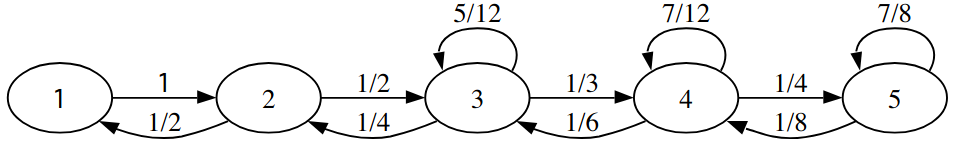
\includegraphics[width = .6\textwidth]{images/markov_rev.png}
			\end{center}
		\end{figure}
	
	
	
		\stepcounter{num} 
	\paragraph{Exercise \thenum.}% (Reversibility)
	Consider a Markov chain on the state space $\{1, 2,\ldots, 7\}$, and transitions given by moving one step clockwise or counterclockwise with equal probabilities. For example, from state 6, the chain moves
	to state 7 or state 5 with probability $0.5$ each; from state 7, the chain moves to state 1
	or state 6 with probability $0.5$ each. 
	The chain starts at state 1.
	\begin{enumerate}
		\item Draw the Markov graph of this chain.
		\item Find the stationary distribution of this chain.
		\item Consider a new chain obtained by unfolding the circle. 
		From state 1 the chain always goes to state 2, and from state 7 the	chain always goes to state 6. 
		Draw the Markov graph and find the new stationary distribution.
	\end{enumerate}
		\begin{figure}[h!]
			\begin{center}
				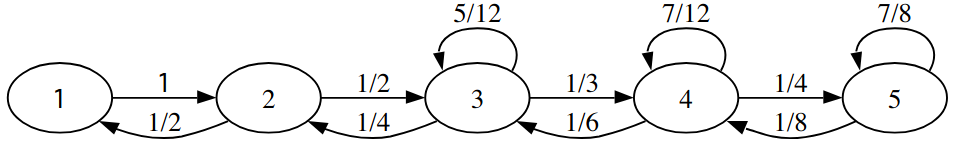
\includegraphics[width = .6\textwidth]{images/markov_rev.png}
			\end{center}
		\end{figure}
	
	
	\stepcounter{num} 
	\paragraph{Exercise \thenum.} (Transition matrix)
		A component of a computer has an active life, measured in discrete units, that is a random variable $T$ where
		$P (T = k) = a_k$ for $k = 1, 2,\ldots$. 
		Suppose one starts with a fresh component and each component is replaced by a new component upon failure. Let $X_n$ be the age of the component in service at time $n$.
		\begin{enumerate}
			\item Let $p_i = P(X_n+1 = i + 1 | X_n = i)$ and $q_i = P (X_n+1 = 0 | X_n = i)$ for all $n$. 
			Write down the stochastic matrix of $\{X_n\}$.
			\item Find $p_i, q_i$ in terms of $a_i$.
		\end{enumerate}
	
	
	\stepcounter{num} 
	\paragraph{Exercise \thenum.}
	There are two urns with a total of 2N distinguishable balls. Initially, the first urn has $N$ white balls and the second urn has $N$ black balls. At each stage, we pick a ball at random from each urn and interchange them. Let $X_n$ be the number of black balls in the first urn at time $n$. 
	This is a Markov chain on the state space $\{0, 1,\ldots, N \}$.
	\begin{enumerate}
		\item Give the transition probabilities of the chain.
		\item Show that $(s_0, s_1,\ldots, s_N)$ where
		\begin{equation}
			s_i = \frac{\binom{N}{i}\binom{N}{N-i}}{\binom{2N}{N}}.
		\end{equation}
		\end{enumerate}
	
	\stepcounter{num} 
	\paragraph{Exercise \thenum.}
	A cat and a mouse move independently back and forth between two rooms. At each
	time step, the cat moves from the current room to the other room with probability 0.8.
	Starting from room 1, the mouse moves to Room 2 with probability 0.3 (and remains
	otherwise). Starting from room 2, the mouse moves to room 1 with probability 0.6 (and
	remains otherwise).
	\begin{enumerate}
		\item Find the stationary distributions of the cat chain and of the mouse chain.
		\item Note that there are 4 possible (cat, mouse) states: both in room 1, cat in room
		1 and mouse in room 2, cat in room 2 and mouse in room 1, and both in room 2.
		Number these cases $1, 2, 3, 4$, respectively, and let $Z_n$ be the number representing the
		(cat, mouse) state at time n. Is $Z_0, Z_1, Z_2,\ldots$ a Markov chain?
		\item Now suppose that the cat will eat the mouse if they are in the same room. 
		We wish to know the expected time (number of steps taken) until the cat eats the mouse for two initial configurations: when the cat starts in room 1 and the mouse starts in room 2, and vice versa. 
		Set up a system of two linear equations in two unknowns whose solution is the desired values.
	\end{enumerate}
	\paragraph{References and acknowledgments:} Introduction to probability (Blitzstein and Huang) - Lisa Ruan - Christy Huo.
	%Lisa Ruan and Christy Huo (ex 2, 3), stat 171 harvard
	\end{document}